\chapter{\sffamily Spatial density fields}

{\bfseries\sffamily Concept.} The idea here is to limit the spread of some abstract spatial parasitic infections through the correct time-dependent resource allocation.

\textcolor{red}{This spatial density field archetype would make sense in simulations of epidemiological processes, ecosystems or even weather systems.}


\section{\sffamily Adapting the probabilistic formalism}

\begin{figure}[h]
\centering
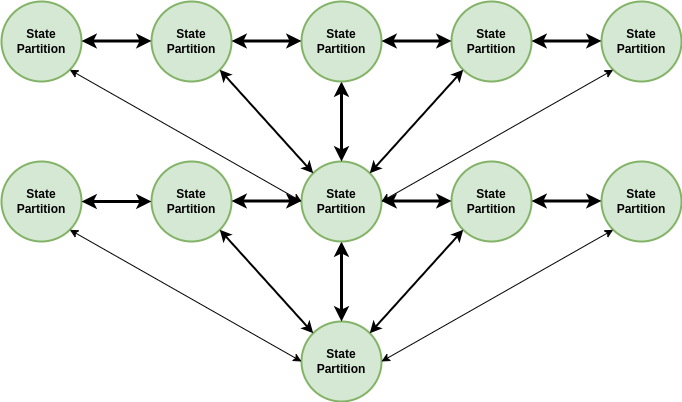
\includegraphics[width=11cm]{images/chapter-7-state-partition-graph.drawio.png}
\caption{State partition graph topology for spatial density field archetypes.}
\label{fig:state-partition-graph-spatial-density-fields}
\end{figure}

Let's by returning to the probabilistic formalism that we introduced earlier and noting that the covariance matrix estimate with elements $C^{ij}_{{\sf t}+1}(z)$ represents a matrix that could get very large, depending on the problem. For example; if we encoded the state of a 2-dimensional spatial field of values into the elements $X^i_{\sf t}$, the number of elements in the covariance matrix $C^{ij}_{{\sf t}+1}(z)$ would scale as $4N^2$ --- where $N$ here is the number of spatial points we wanted to encode. 

One solution to this scaling problem is to exploit the fact that, in many spatial processes, the proximity of points can strongly determine how correlated they are. Hence, for pairwise distances further than some threshold, the covariance matrix elements should tend towards 0. If we were to place points along the diagonal of $C^{ij}_{{\sf t}+1}(z)$ in order of how close they are to each other, this threshold would then be represented as a \emph{banded matrix}. We have illustrated such a matrix in Fig.~\ref{fig:banded-matrix} in which the `bandwidth' is defined as the number of diagonals one needs to traverse from the main diagonal before encountering a diagonal of 0s.

\begin{figure}[h]
\centering
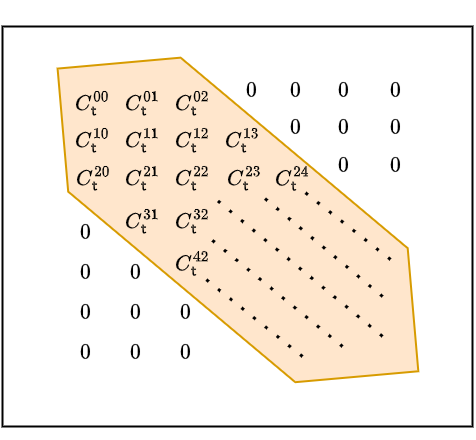
\includegraphics[width=9cm]{images/chapter-7-banded-matrix.drawio.png}
\caption{An illustration of a banded covariance matrix with a bandwidth of 2.}
\label{fig:banded-matrix}
\end{figure}

\textcolor{red}{
\begin{itemize}
\item{Full sim: fully individual-based spatial stochastic model}
\item{Inference model: spatial mean field inference features using the probabilistic reweighting + exponentially-weighted nonlinear features}
\item{Also use the likelihood-free inference model and amortized sim inference model.}
\end{itemize}
}

\textcolor{red}{
\begin{itemize}
\item{At some point it might be sensible to move into the Fourier domain here --- at least for derivations and calculations. Probably more intuitive for the reader to keep it mostly in real space though if possible.} 
\item{The extra detail that's also needed here is to consider how we encode a 2-dimensional spatial process into our state vector, and how the elements of the resulting state vector might be correlated to one another depending on their spatial proximity. If we start with a Markovian Gaussian random field, we can derive the Mat\'{e}rn kernel over these spatial coordinates in order to correlate the state vectors in such a way.} 
\item{Also look into the Radial Basis Function (RBF) and higher-order derived kernels based on DALI expansion~\cite{sellentin2014breaking} in order to try and capture non-Gaussianity.}
\end{itemize}
}
